\documentclass{beamer}

\usetheme{avad}

\usepackage[utf8]{inputenc}
\usepackage{amsmath,amssymb}
\usepackage{array,multirow}

\graphicspath{%
{figs/}%
}



%%%%%%%%%%%%%%%%%%%%%%%%%%%%%%%%%%%%%%%%%%%%%%%%%%%%%%%%%%%%%%%%%%%%%%%%%%%%%%%%
%%%%%%%%%%%%%%%%%%%%%%%%%%%%%%%%%%%%%%%%%%%%%%%%%%%%%%%%%%%%%%%%%%%%%%%%%%%%%%%%
\begin{document}

%%%%%%%%%%%%%%%%%%%%%%%%%%%%%%%%%%%%%%%%%%%%%%%%%%%%%%%%%%%%%%%%%%%%%%%%%%%%%%%%
\title{Wissenschaftliche Erkenntnis, Reproduzierbarkeit und praktische Lösungen
in der Akustik}
\subtitle{Hagen Wierstorf$\;^1$, Sascha Spors$\,^2$, Matthias Geier$\,^2$\\%
          \vspace{0.5cm}%
          \footnotesize{%
          $^1\,$Filmuniversität Bablesberg \emph{KONRAD WOLF}\\%
          $^2\,$Institut für Nachrichtentechnik, Universität Rostock}}
\author{Hagen Wierstorf$\,$\inst{1} \and
        Sascha Spors\inst{2} \and
        Matthias Geier\inst{2}}
\institute{\inst{1} Filmuniversität Bablesberg \emph{KONRAD WOLF}\\
           \inst{2} Institut für Nachrichtentechnik, Universität Rostock}
\date{07.03.2017}
\maketitle

%%%%%%%%%%%%%%%%%%%%%%%%%%%%%%%%%%%%%%%%%%%%%%%%%%%%%%%%%%%%%%%%%%%%%%%%%%%%%%%%
\begin{frame}{Motivation}

    \textbf{Reproduzierbarkeitskrise}

    \begin{itemize}
        \item Psychologie: nur $47$\% reproduzierbare Studien ($N=100$)\footnote{%
            Open Science Collaboration (2015), \emph{Science},
            doi:10.1126/science.aac4716}
        \item Pharmazie: nur $21$\% reproduzierbare Studien ($N=120$)\footnote{%
            Prinz, et al. (2011), \emph{Nature Reviews Drug Discovery},
            doi:10.1038/nrd3439-c1}\textsuperscript{,}\footnote{%
            Begley \& Ellis (2012), \emph{Nature},
            doi:10.1038/483531a}
        \item Genetik: $44$\% reproduzierbare Datenanalyse ($N=18$)\footnote{%
            Ioannidis, et al. (2009), \emph{Nature Genetics},
            doi:10.1038/ng.295}
    \end{itemize}

    Noch Links zu den gerade laufenden Studien/initiativen hinzufügen.

\end{frame}

%%%%%%%%%%%%%%%%%%%%%%%%%%%%%%%%%%%%%%%%%%%%%%%%%%%%%%%%%%%%%%%%%%%%%%%%%%%%%%%%
\begin{frame}{Wissenschaftliche Methode}

    \begin{itemize}
        \item \textbf{Deduktiv:} \\
            \small{Dachs ist ein Säugetier\\%
                   Dieter ist ein Dachs\\%
                   $\Rightarrow$ Dieter ist ein Säugetier}
    \end{itemize}
    \begin{itemize}
        \item \textbf{Induktiv:} \\
            \small{Medikament hatte keine Nebenwirkung an $100\,000$ getesteten
                   Menschen.\\%
                   Kann sicher verwendet werden.}
    \end{itemize}
    \begin{itemize}
        \item \textbf{Computer Simulation:} \\
            \small{Numerik und große Datensätze (Beispiel?)}
            Zitat Donoho (und Stodden)
            $\Rightarrow$ heutige Praxis erzeugt in den meisten Fällen keine
            zuverlässigen (reliable) Ergebnisse

    \end{itemize}

\end{frame}

%%%%%%%%%%%%%%%%%%%%%%%%%%%%%%%%%%%%%%%%%%%%%%%%%%%%%%%%%%%%%%%%%%%%%%%%%%%%%%%%
\begin{frame}{Wann ist etwas Wissenschaft?}

    Überprüfung einer Aussage durch \textbf{Falsifizierbarkeit}
    \begin{quote}
        If it disagrees with experiment, it's wrong. In that simple statement is
        the key to science.
    \end{quote}

    {\ft\hfill R. Feynman zitiert nach T. Lewens (2015)}

    \vspace{1cm}

    \begin{itemize}
        \item Nicht automatisch Widerlegung einer Theorie (Gran Sasso, 2011)
        \item Kann als Abgrenzung von Pseudowissenschaften verwendet werden
            (Astronomie)
        \item \textbf{Reproduzierbarkeit} von Ergebnissen wichtig
    \end{itemize}

\end{frame}

%%%%%%%%%%%%%%%%%%%%%%%%%%%%%%%%%%%%%%%%%%%%%%%%%%%%%%%%%%%%%%%%%%%%%%%%%%%%%%%%
\begin{frame}{Gründe für Nicht-Reproduzierbarkeit}

    \vspace{-0.5cm}

    \begin{figure}
        \centering
        \begin{tikzpicture}
            \draw (-4, 2.0) node {
\includegraphics[width=2cm]{data_dredging}};
            \draw (-4, 1.1) [text width=4cm,align=center,anchor=north] node
                {\textbf{Datenmelken}\\
                 \sm Suchen nach signifikanten Ergebnissen\par};
            \draw ( 0, 2.0) node {
\includegraphics[width=2cm]{omitting_null_results}};
            \draw ( 0, 1.1) [text width=4cm,align=center,anchor=north] node
                {\textbf{Positiver Bias}\\
                 \sm Nur positive Ergebnisse werden publiziert\par};
            \draw ( 4, 2.0) node {
\includegraphics[width=2cm]{underpowered_study}};
            \draw ( 4, 1.1) [text width=4cm,align=center,anchor=north] node
                {\textbf{Teilnehmerzahl}\\
                 \sm Zu wenig statistische Power für Effekstärke\par};
            \draw (-4,-1.4) node {
\includegraphics[width=2cm]{errors}};
            \draw (-4,-2.3) [text width=4cm,align=center,anchor=north] node
                {\textbf{Fehler}\\
                 \sm Technische oder Programmierfehler\par};
            \draw ( 0,-1.4) node {
\includegraphics[width=2cm]{underspecified_method}};
            \draw ( 0,-2.3) [text width=4cm,align=center,anchor=north] node
                {\textbf{Unklare Methode}\\
                 \sm Methode ungenügend beschrieben\par};
            \draw ( 4,-1.4) node {
\includegraphics[width=2cm]{weak_experimental_design}};
            \draw ( 4,-2.3) [text width=4cm,align=center,anchor=north] node
                {\textbf{Schlechtes Design}\\
                 \sm Experiment hat systematische Fehler\par};
        \end{tikzpicture}
    \end{figure}

    {\ft\hfill Abbildung basierend auf The Academy of Medical Sciences (2015)}

\end{frame}

%%%%%%%%%%%%%%%%%%%%%%%%%%%%%%%%%%%%%%%%%%%%%%%%%%%%%%%%%%%%%%%%%%%%%%%%%%%%%%%%
\begin{frame}{Statistik}

    Gehe auf folgende Punkte ein

    \begin{itemize}
        \item p-Hacking
        \item Wie Wahrscheinlich sind false-positives
        \item Vergleich Neurowissenschaften vs. Teilchenphysik
        \item \dots
    \end{itemize}

\end{frame}

%%%%%%%%%%%%%%%%%%%%%%%%%%%%%%%%%%%%%%%%%%%%%%%%%%%%%%%%%%%%%%%%%%%%%%%%%%%%%%%%
\begin{frame}{Statistik}

    \begin{figure}
        \centering
        \begin{tikzpicture}
            \only<1>{\draw (0,0) node {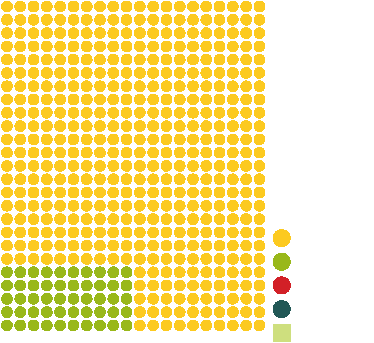
\includegraphics[width=7cm]{stat1_1}};}
            \only<2>{\draw (0,0) node {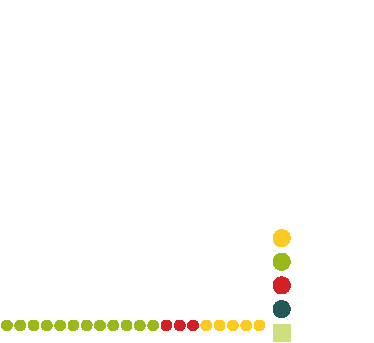
\includegraphics[width=7cm]{stat1_2}};}
            \only<3>{\draw (0,0) node {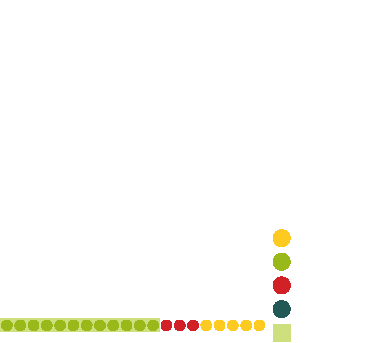
\includegraphics[width=7cm]{stat1_3}};}
            \draw (2.0,2.5) [right] node {\sm 20 Hypothesen};
            \draw (2.0,2.0) [right] node {\sm Power: $0.8$};
            \draw (2.0,1.5) [right] node {\sm $p = 0.05$};
            \draw (1.9,-1.24) [right] node {\sm unwahr};
            \draw (1.9,-1.70) [right] node {\sm wahr};
            \draw (1.9,-2.16) [right] node {\sm falsch negativ};
            \draw (1.9,-2.62) [right] node {\sm falsch positiv};
            \draw (1.9,-3.08) [right] node {\sm publiziert};
        \end{tikzpicture}
    \end{figure}

\end{frame}

%%%%%%%%%%%%%%%%%%%%%%%%%%%%%%%%%%%%%%%%%%%%%%%%%%%%%%%%%%%%%%%%%%%%%%%%%%%%%%%%
\begin{frame}{Statistik}

    \begin{figure}
        \centering
        \begin{tikzpicture}
            \only<1>{\draw (0,0) node {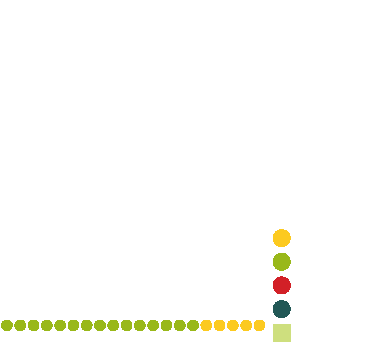
\includegraphics[width=7cm]{stat2_1}};}
            \only<2>{\draw (0,0) node {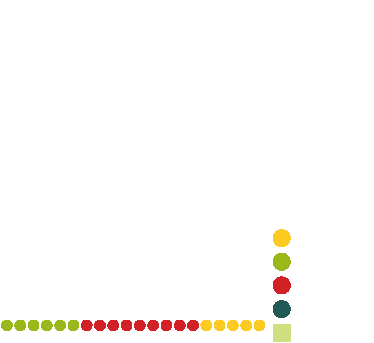
\includegraphics[width=7cm]{stat2_2}};}
            \only<3>{\draw (0,0) node {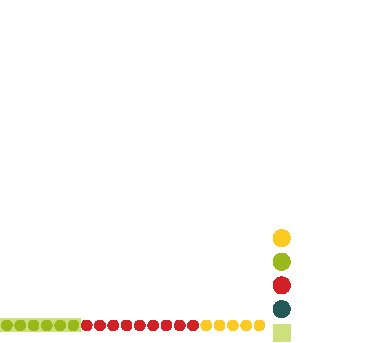
\includegraphics[width=7cm]{stat2_3}};}
            \draw (2.0,2.5) [right] node {\sm 20 Hypothesen};
            \draw (2.0,2.0) [right] node {\sm Power: $0.4$};
            \draw (2.0,1.5) [right] node {\sm $p = 0.05$};
            \draw (1.9,-1.24) [right] node {\sm unwahr};
            \draw (1.9,-1.70) [right] node {\sm wahr};
            \draw (1.9,-2.16) [right] node {\sm falsch negativ};
            \draw (1.9,-2.62) [right] node {\sm falsch positiv};
            \draw (1.9,-3.08) [right] node {\sm publiziert};
        \end{tikzpicture}
    \end{figure}

\end{frame}

%%%%%%%%%%%%%%%%%%%%%%%%%%%%%%%%%%%%%%%%%%%%%%%%%%%%%%%%%%%%%%%%%%%%%%%%%%%%%%%%
\begin{frame}{Statistik}

    \begin{figure}
        \centering
        \begin{tikzpicture}
            \only<1>{\draw (0,0) node {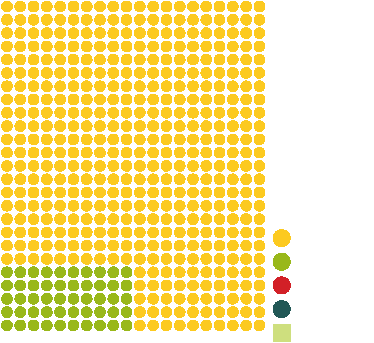
\includegraphics[width=7cm]{stat3_1}};}
            \only<2>{\draw (0,0) node {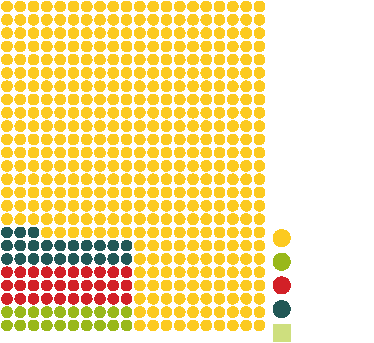
\includegraphics[width=7cm]{stat3_2}};}
            \only<3>{\draw (0,0) node {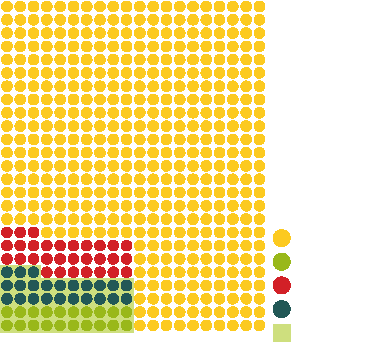
\includegraphics[width=7cm]{stat3_3}};}
            \draw (2.0,2.5) [right] node {\sm 500 Hypothesen};
            \draw (2.0,2.0) [right] node {\sm Power: $0.4$};
            \draw (2.0,1.5) [right] node {\sm $p = 0.05$};
            \draw (1.9,-1.24) [right] node {\sm unwahr};
            \draw (1.9,-1.70) [right] node {\sm wahr};
            \draw (1.9,-2.16) [right] node {\sm falsch negativ};
            \draw (1.9,-2.62) [right] node {\sm falsch positiv};
            \draw (1.9,-3.08) [right] node {\sm publiziert};
        \end{tikzpicture}
    \end{figure}

\end{frame}

%%%%%%%%%%%%%%%%%%%%%%%%%%%%%%%%%%%%%%%%%%%%%%%%%%%%%%%%%%%%%%%%%%%%%%%%%%%%%%%%
\begin{frame}{Auswege}

    \begin{tabular}{>{\raggedright}p{5.5cm}l}
        \textbf{Open Science} & \multirow{2}{2cm}{%
            
\includegraphics[width=1cm]{data_dredging}
            
\includegraphics[width=1cm]{omitting_null_results}
            
\includegraphics[width=1cm]{errors}
            
\includegraphics[width=1cm]{underspecified_method}
            
\includegraphics[width=1cm]{weak_experimental_design}} \\
        Daten, Software und Methoden & \\[1em]
        \textbf{Pre-Registrierung} & \multirow{2}{2cm}{%
            
\includegraphics[width=1cm]{data_dredging}
            
\includegraphics[width=1cm]{omitting_null_results}
            
\includegraphics[width=1cm]{underpowered_study}
            
\includegraphics[width=1cm]{underspecified_method}
            
\includegraphics[width=1cm]{weak_experimental_design}} \\
        des Versuches (und Review) & \\[1em]
        \textbf{Zusammenarbeit} & \multirow{2}{*}{%
            
\includegraphics[width=1cm]{underpowered_study}
            
\includegraphics[width=1cm]{underspecified_method}
            
\includegraphics[width=1cm]{weak_experimental_design}} \\
        unterschiedlicher Arbeitsgruppen & \\[1em]
        \textbf{Post-publication review} & \multirow{2}{*}{%
            
\includegraphics[width=1cm]{underspecified_method}
            
\includegraphics[width=1cm]{weak_experimental_design}} \\
        Diskussion und Verbesserungen & \\[1em]
        \textbf{Statistische Fortbildung} & \multirow{2}{*}{%
            
\includegraphics[width=1cm]{data_dredging}
            
\includegraphics[width=1cm]{omitting_null_results}} \\
        & \\
    \end{tabular}

\end{frame}

%%%%%%%%%%%%%%%%%%%%%%%%%%%%%%%%%%%%%%%%%%%%%%%%%%%%%%%%%%%%%%%%%%%%%%%%%%%%%%%%
\begin{frame}{Beispiel: Open Science in der Akustik}

    Studien-Ziel: Qualität verschiedener Audiowiedergabeverfahren miteinander
    vergleichen

    \textbf{Daten}
    \begin{itemize}
        \item Ausgangs Audiomaterial
        \item Gemischtes Audiomaterial/Lautsprechersignale
        \item HRTFs (bei binauraler Simulation der Lautsprecher)
        \item Roh-Daten aus dem Hörversuch
    \end{itemize}

    \textbf{Software}
    \begin{itemize}
        \item Implementation Wiedergabeverfahren (z.B. Wellenfeldsynthese)
        \item Implementation Binauralsynthese
        \item \dots
    \end{itemize}

    \textbf{Methoden}
    \begin{itemize}
        \item GUI für den Hörversuch
        \item Instruktionen für die Versuchspersonen
        \item Statistische Auswertung
    \end{itemize}

\end{frame}

%%%%%%%%%%%%%%%%%%%%%%%%%%%%%%%%%%%%%%%%%%%%%%%%%%%%%%%%%%%%%%%%%%%%%%%%%%%%%%%%
\begin{frame}{Beispiel: Open Science in der Akustik}

    \begin{itemize}
        \item Erwähnen, dass es interessant wäre dies direkt ins Paper zu
            integrieren ($\Rightarrow$ Jupyter)
        \item Beispiel zeigen wie die einzelnen Punkte gelöst worden sind
        \item Wie am besten? Mit verweisen auf veröffentlichte Software/Daten
            und Screenshots?
    \end{itemize}

\end{frame}

\end{document}
